%%
%% sample document for AAMAS'19 conference
%%
%% modified from sample-sigconf.tex
%%
%% see ACM instructions acmguide.pdf
%%
%% AAMAS-specific questions? F.A.Oliehoek@tudelft.nl
%%

\documentclass[sigconf]{aamas}  % do not change this line!

%% your usepackages here, for example:
\usepackage{booktabs}

%% do not change the following lines
\usepackage{flushend}
%\setcopyright{ifaamas}  % do not change this line!
\acmDOI{}  % do not change this line!
\acmISBN{}  % do not change this line!
\acmConference[AASMA'23]{AASMA Project, IST}{2023}{Lisbon, Portugal}  % do not change this line!
\acmYear{2023}  % do not change this line!
\copyrightyear{2023}  % do not change this line!
\acmPrice{}  % do not change this line!

%% the rest of your preamble here


%%%%%%%%%%%%%%%%%%%%%%%%%%%%%%%%%%%%%%%%%%%%%%%%%%%%%%%%%%%%%%%%%%%%%%%%%%%%%%%%%%%%%%%%%%%%%%%%%%%%%%%%%

\begin{document}

\title{Competitive Multiplayer Snake Game}  % put your title here!
%\titlenote{Produces the permission block, and copyright information}

% AAMAS: as appropriate, uncomment one subtitle line; check the CFP
%\subtitle{Extended Abstract}
%\subtitle{Blue Sky Ideas Track}
%\subtitle{JAAMAS Track}
%\subtitle{Demonstration}
%\subtitle{Doctoral Consortium}

% AAMAS: submissions are anonymous for most tracks
\subtitle{Group 38 - Project Report - Autonomous Agents and Multi-Agent Systems}

%% example of author block for camera ready version of accepted papers: don't use for anonymous submissions
%
\author{Simão Paiva}
\affiliation{%
  \institution{Instituto Superior Técnico}
  \city{Oeiras}
  \country{Portugal}
}
\email{simao.paiva@tecnico.ulisboa.pt}

\author{David Duque}
\affiliation{
  \institution{Instituto Superior Técnico}
  \city{Oeiras}
  \country{Portugal} 
}
\email{david.f.s.duque@tecnico.ulisboa.pt}
%
%\author{Lars Th{\o}rv{\"a}ld}
%\authornote{This author is the
%  one who did all the really hard work.}
%\affiliation{%
%  \institution{The Th{\o}rv{\"a}ld Group}
%  \streetaddress{1 Th{\o}rv{\"a}ld Circle}
%  \city{Hekla} 
%  \country{Iceland}}
%\email{larst@affiliation.org}
%
%\author{Valerie B\'eranger}
%\affiliation{%
%  \institution{Inria Paris-Rocquencourt}
%  \city{Rocquencourt}
%  \country{France}
%}
%\author{Aparna Patel} 
%\affiliation{%
% \institution{Rajiv Gandhi University}
% \streetaddress{Rono-Hills}
% \city{Doimukh} 
% \state{Arunachal Pradesh}
% \country{India}}
%\author{Huifen Chan}
%\affiliation{%
%  \institution{Tsinghua University}
%  \streetaddress{30 Shuangqing Rd}
%  \city{Haidian Qu} 
%  \state{Beijing Shi}
%  \country{China}
%}
%
%\author{Charles Palmer}
%\affiliation{%
%  \institution{Palmer Research Laboratories}
%  \streetaddress{8600 Datapoint Drive}
%  \city{San Antonio}
%  \state{Texas} 
%  \postcode{78229}}
%\email{cpalmer@prl.com}
%
%\author{John Smith}
%\affiliation{\institution{The Th{\o}rv{\"a}ld Group}}
%\email{jsmith@affiliation.org}
%
%\author{Julius P.~Kumquat}
%\affiliation{\institution{The Kumquat Consortium}}
%\email{jpkumquat@consortium.net}
%
%% The example's default list of authors is too long for headers
%\renewcommand{\shortauthors}{B. Trovato et al.}


\begin{abstract}  % put your abstract here!
In this project, we designed and implemented a simulation environment for the game of Snake with multiple independent agents.
Our approach involves developing independent AI agents to control individual snakes in the game and compete for resources (food).
We investigate the effectiveness of different algorithms for the agents, explore the impact of different factors,
such as the size of the environment or the number and type of agents, on their performance, and also explore the potential of
combining multiple algorithm outputs to make decisions.
Our expected contributions include the development of a competitive and scalable multi-agent system, as well as insights
into the effectiveness of different algorithms and their combinations in a multi-agent setting.
\end{abstract}


% \keywords{AAMAS; ACM proceedings; \LaTeX; text tagging}  % put your semicolon-separated keywords here!

\maketitle


%%%%%%%%%%%%%%%%%%%%%%%%%%%%%%%%%%%%%%%%%%%%%%%%%%%%%%%%%%%%%%%%%%%%%%%%%%%%%%%%%%%%%%%%%%%%%%%%%%%%%%%%%
%% start of main body of paper

\graphicspath{ {./img/} }
\section{Introduction}
In Computer Science, the game of Snake has long served as a famous illustration of how algorithms, data structures, and AI
work. However, the majority of Snake implementations are made for a single player, whose only objective is to survive for
as long as feasible, and grow as big as possible.
In fact, the Classical Snake Game is a “solved” game, in the sense that there are known algorithms that are able to
always win the game~\cite{ClassicSnakeGame}.

By integrating multiple (that is, at least two) snakes, each controlled by an AI agent, that compete for
points (food) in a shared environment, this project is an expansion of the game of Snake. As a result, the game gets a new layer
of complexity, which presents an intriguing challenge for agents to develop winning methods against each other.

In this case, the problem is to create a group of autonomous agents, each in control of a single snake, to compete with other
snakes for points (food) in a shared environment. They should be able to perceive their surroundings, including the
locations of other snakes and food, and make decisions about where to move their snake based on this understanding.
The objective is for each agent to score more points than the other agents over the course of a set amount of time, either by
increasing the number of points that its snake accrues, eliminating the opposition, or doing both at once.

This has relevance, as many real-world applications, such as robotics, self-driving cars, and games, are concerned with the
problem of designing AI agents that can compete in complex, dynamic and clearly non-deterministic environments. The game of
Snake, in particular, with multiple independent agents, provides an intriguing and challenging environment for developing and
testing new AI algorithms. Learning effective strategies for competing against other agents has potential applications in a
variety of fields, including finance and marketing.

Within this project, we have multiple objectives, such as creating a simulation environment for the game of Snake that includes
multiple independent agents, autonomous agents to control individual snakes in the game and get them to compete for points,
examine the effectiveness of various algorithms for agents, and investigate the effect of various factors on the performance
of autonomous agents, such as the size of the environment and the number of agents, and lastly explore the possibility of making

decisions by combining the outputs of multiple algorithms. This may result in better performance than using a single algorithm alone.

\subsection{Related Work}

Our project shares some similarities with the paper \textit{“Snake game AI: Movement rating functions and evolutionary algorithm-based
optimization”}~\cite{SnakeGameNaturalSelection}. Both projects involve developing agents to control snakes in the game of Snake, albeit in different variations.
However, while the authors of that article focus on developing a controller based on movement rating functions and using an evolutionary algorithm to
find a set of `good' weight values, this project focuses on developing independent agents that learn to compete for points using different algorithms,
and exploring the impact of different factors on their performance.

Our project and the paper titled \textit{"Training a Reinforcement Learning Agent based on XCS in a Competitive Snake Environment"}~\cite{SnakeGameXCS}
share some similarities in that both involve developing AI agents to compete in a Snake Game environment involving multiple agents.
This project differs from the XCS-based approach in that our environment rewards not only for collecting points, but also for taking down other agents,
by creating an alggomeration of food near where other agents died, therefore possibly incentivizing strategies other than `going for the food'.
It is expected that more interaction between agents happens in this project, as it is possible to be the most efficient way for an agent to win.

The variation to the environment designed for this project (compared to the classical Snake Game) is inspired on \textit{slither.io}, a multiplayer game
which is itself a variation of the Classic Snake Game.

\section{Approach}
In this section, we will explain the environment, how the agents interact with it, and the mechanics of the game itself.
\subsection{The Environment}

The game environment is composed of a grid of fixed area ($\texttt{a} \times \texttt{b}$ squares, where \texttt{a} and \texttt{b} are set before the game begins).
The number of agents in the environment may be arbitrarily high, but for the sake of getting appropriate results, the maximum number of agents the environment
can adequately hold scales with its own area.
The time in the game is measured in steps, where $\texttt{steps} \in \mathbb{Z}^0_+$.

\begin{figure}
  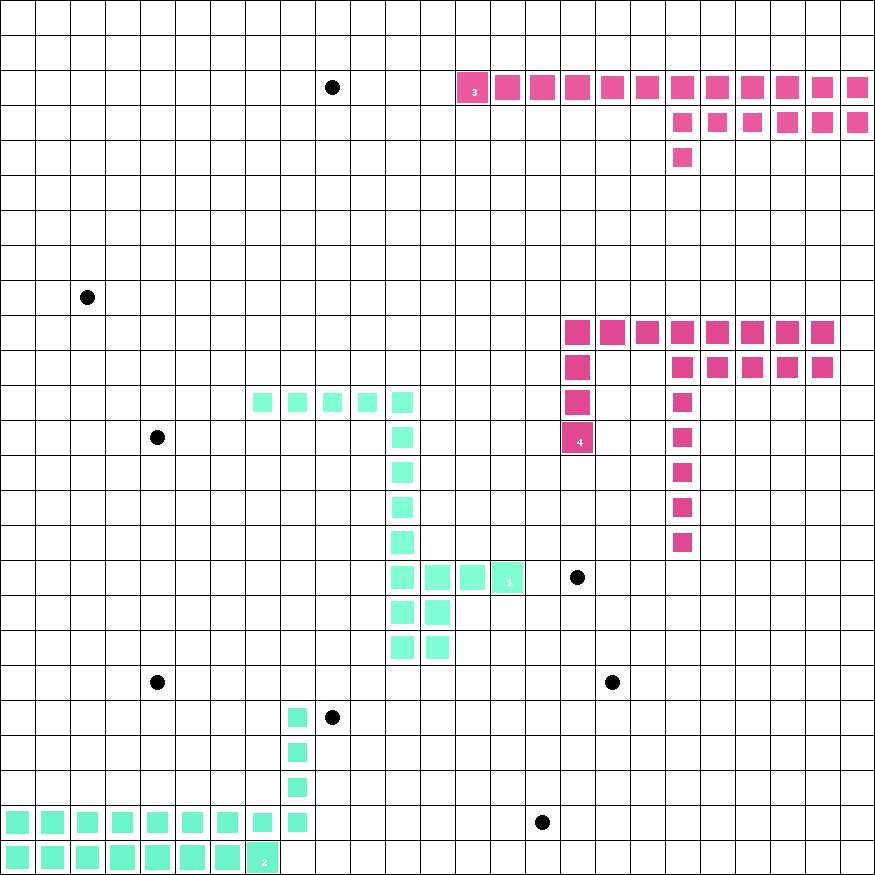
\includegraphics[height=2.8in, width=2.8in]{sample_env}
  \caption{A representation of the game environment in a certain point in time. There are four agents in this game. The black dots represent the food points.}
\end{figure}

Unlike the Classical Snake Game (which only contains one food point at any point in time), the environment may contain any number of food points, up to the entire area
of the environment not already occupied by the snakes. Every step, there is a certain probability of a new food point appearing on the environment,
calculated the following way\footnote{
  \textbf{$food_{av}$} = food currently available in the environment; \textbf{$food_{eq}$} = food equilibrium of the environment,
  which can be defined as a function of the environment total or available area. The experiments in this report use $food_{eq}(area_{av}) = \frac{\sqrt{area_{av}}}{2}$ as the
  equilibrium function.
}:

\begin{flalign*}
  P(\text{food appearing}) = \begin{cases}
    0 & \text{if } food_{av} \ge food_{eq}\\
    \frac{food_{eq} - food_{av}}{food_{eq}} & \text{otherwise}
  \end{cases}
\end{flalign*}

The location of the food points generated this way is randomly determined, tendentially evenly across the environment.

At the start of the game, the agents are placed at random locations, so that they do not intersect with eachother. All snakes start with a length of 3.
Eating a food point increases the length of the agent by 1.
Every move, each agent must take one of three actions in this environment - \texttt{FORWARD}, \texttt{LEFT} or \texttt{RIGHT}. These actions are
relative to the orientation of their head - for example: if it is
pointed to the right edge of the map, the \texttt{RIGHT} action will make
it head towards the bottom edge of the environment.
Agents have knowledge of nearly the entire environment at any point in
time, including their own position and length, the number and
location of food points, obstacles (their own body and the body of
the other agents). Agents do not have knowledge about where or when
a new food point will be naturally created (or about the food equilibrium),
nor what kind or what algorithm other agents are running.

An agent is removed from the game (that is, it “dies”), if one of the following conditions happens:

\begin{itemize}
  \item The agent's head collides with the body (excluding the head) of any snake, including its own;
  \item The agent's head collides with the head of another agent (in which both agents are removed from the game);
  \item The agent's head collides with any edge of the environment.
\end{itemize}

Should an agent be removed from the game, its body is partly replaced with food points (every other unit of the agent's body is replaced with a food block,
while the other half is replaced with empty spaces). This mechanic may encourage alternative win conditions: actively forcing another agent to die instead
of trying to preserve its own length may be a viable strategy, even in games with more than 2 agents.

The game ends as soon as at least one of the following conditions is met:
\begin{itemize}
  \item The step limit (may be determined as a function of the area of the environment
\footnote{In the experiments present in this report, the step limit is equal to the total area of the environment: $\texttt{a} \times \texttt{b}$})
  is reached. The winner is the agent with the greatest body length;
  \item There is 1 or less agent remaining in the game (last man standing). The sole remaining agent (if it exists)
  is declared the winner. If there are no agents (because the last two agents collided head-on or oterwise died at the same time),
  there is no winner and the game is declared a draw.
\end{itemize}

\subsection{The Agents}

The agents may be implemented in any algorithm that is able to navigate through a grid.

\subsubsection{Sensors}
All agents get an observation $(\texttt{a},\texttt{b},i_n,S,D,F)$ of the entire environment every step, where:
\begin{itemize}
  \item $(\texttt{a}, \texttt{b}) \text{ is the shape of the environment grid;}$
  \item $i_n \text{ is the agent } n \text{'s own identifier;}$
  \item $S \text{ is the position of all snakes' bodies;}$
  \item $D \text{ is the direction of all agents' heads;}$
  \item $F \text{ is the position of all food points in the environment.}$
\end{itemize}

\subsubsection{Actuators}
Agents have only one actuator, which always outputs one of the following values every step:
\begin{itemize}
  \item \texttt{LEFT}
  \item \texttt{FORWARD}
  \item \texttt{RIGHT}
\end{itemize}

\section{Evaluation Methodology}
For the evaluation of the agents, multiple different scenarios are set up.
A scenario\footnote{While the behavior of the environments remain similar in quality,
they end up differing in quantity in some metric (area, food spawn rate, etc.), so formally
two different tuples $(\texttt{a},\texttt{b},food_{eq},step\_limit,A)$ are two different environments entirely.}
is a tuple $(\texttt{a},\texttt{b},food_{eq},step\_limit,A,n_{episodes})$ where:

\begin{itemize}
  \item $(\texttt{a}, \texttt{b}) \text{ is the shape of the environment grid;}$
  \item $food_{eq}: area_{av}, area_{total} \rightarrow \mathbb{R}^+ \text{ }$ is a food equilibrium function;
  \item $step\_limit \text{ }$ is the maximum number of steps each episode can take;
  \item $A \text{ is the set of the agents that will play the game;}$
  \item $n_{episodes} \text{ is the number of episodes to run.}$
\end{itemize}

In practice, for the scenarios we're presenting, $food_{eq}$ is the same function for all of them,
while $step\_limit$ is defined as a function of $(\texttt{a}, \texttt{b})$. Therefore, and to simplify,
we'll present the scenarios as $(\texttt{a},\texttt{b},A,n_{episodes})$ instead.

In each episode, at least two agents (which may be of the same type or different ones) will be sharing the same
grid and resources, however, their performance as an agent type will be measured as a whole.

The two main performance measurements we are taking are:

\begin{itemize}
  \item The evolution of the agent's length over time (how fast can the agent aggregate resources?);
  \item The evolution of the number of agents still alive over time\footnote{
In this statistical evaluation, an agent that was alive in the episode's terminal step is considered to be alive even after the episode is over.
For example: the last man standing at the step 200 of a certain episode will still
be considered `alive' in step 250.} (how capable is the agent of surviving?).
\end{itemize}

\section{Agents and Comparisons}

\subsection{Random Agent}

\begin{figure}
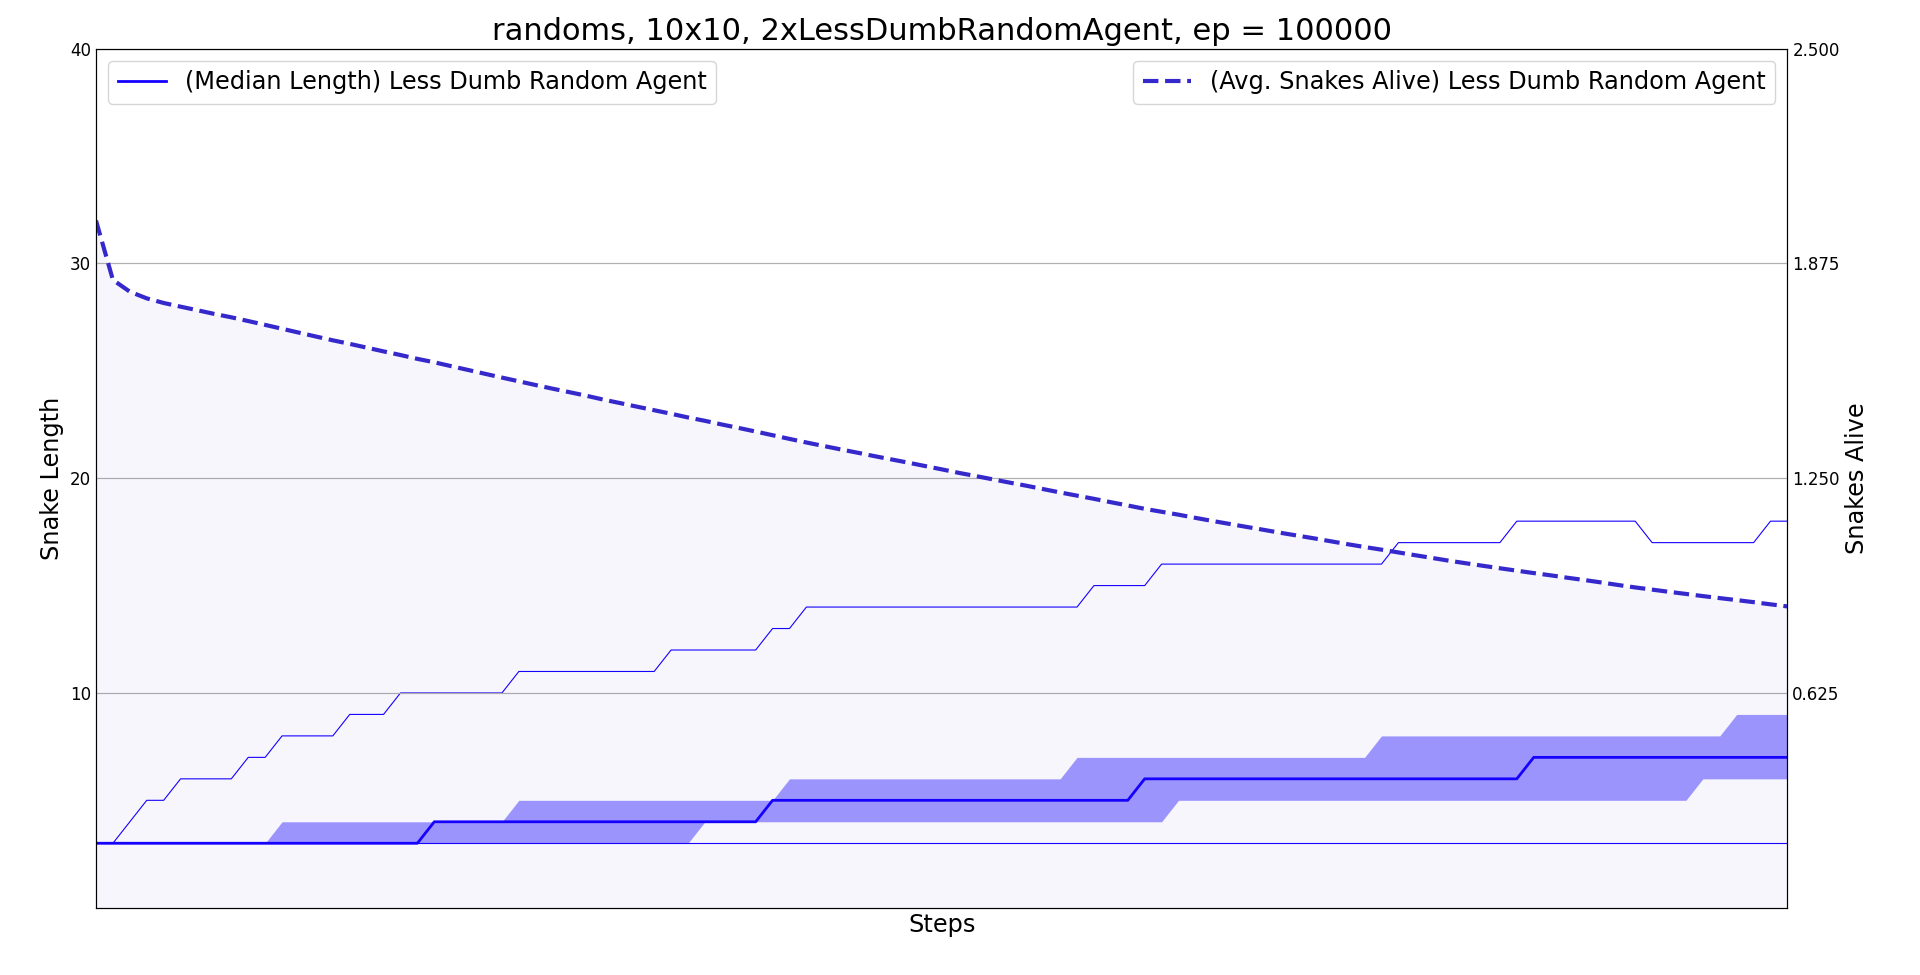
\includegraphics[height=1.6in]{plot_randoms}
\caption{Evolution of the length and population of the Random Agent over time.}
\end{figure}

The Random Agent is a purely reactive agent, in the sense it doesn't actually attempt to plan anything.
It checks first if there are any actions that are nearly-guaranteed to make it die (for example, it will not consider steering left into it's own body).
But like the name implies, it just randomly executes one of the three outputs its actuator offers (\texttt{LEFT}, \texttt{FORWARD}, \texttt{RIGHT}).

The unimpressive results plotted on Figure~\ref{fig_plot_randoms} are therefore not all that surprising: When playing randomly,
the longer the snake is, the more likely it is for it to back itself into a corner, and die by hitting itself because it simply had nowhere else to go.

\subsection{A* Searching Agent}

The A* (A-Star) Searching aims to find the shortest path between start and finish. In the context of this project, this algorithm was used mainly to guide
the agents (read, the snakes) to their destination (the food points). While all of our agents base themselves on this algorithm, they work slightly
differently from eachother.

\subsection{Nearest Food}

In this case, the agent marches towards the food, albeit somewhat blindly. It's gameplan is to reach to it's target as soon as possible. However, this may
not always go as planned. Somebody else may get to that food first, or maybe simply another agent has decided to cross its path.
Therefore, it's unavoidable that the agent needs to re-compute the path to its goal every time, so that it does not inadvertently crash into somebody else.

The agent also re-evaluates its goal when:
\begin{itemize}
  \item It achieves it's original goal (get to a certain food point);
  \item The food point was consumed by another agent or has otherwise disappeared;
  \item Every $x$ moves\footnote{We defined $x = 5$ steps for this project.}.
\end{itemize}

This agent, while it does have a slightly bit more planning capability than the random agent mentioned above, most of its features are still reactive
(it still bases all its decisions on the moment $n$).

Regardless, the by looking at the Figure~\ref{fig_plot_basic4}, we can naturally see that the agent's capability of finding food is orders of magnitude better
than the one of the Random Agent. It can be argued that its survivability is lower because in bigger environments where the food is more spread out,
the Random Agent is able to keep going in circles without actually growing or catching food, and as such it's harder for it to end up colliding with itself.

In fact, we see that the median of the length of the Random Agent never really surpasses 10, while the A* Searcher is able to, on average, grow linearly with time.

\begin{figure}
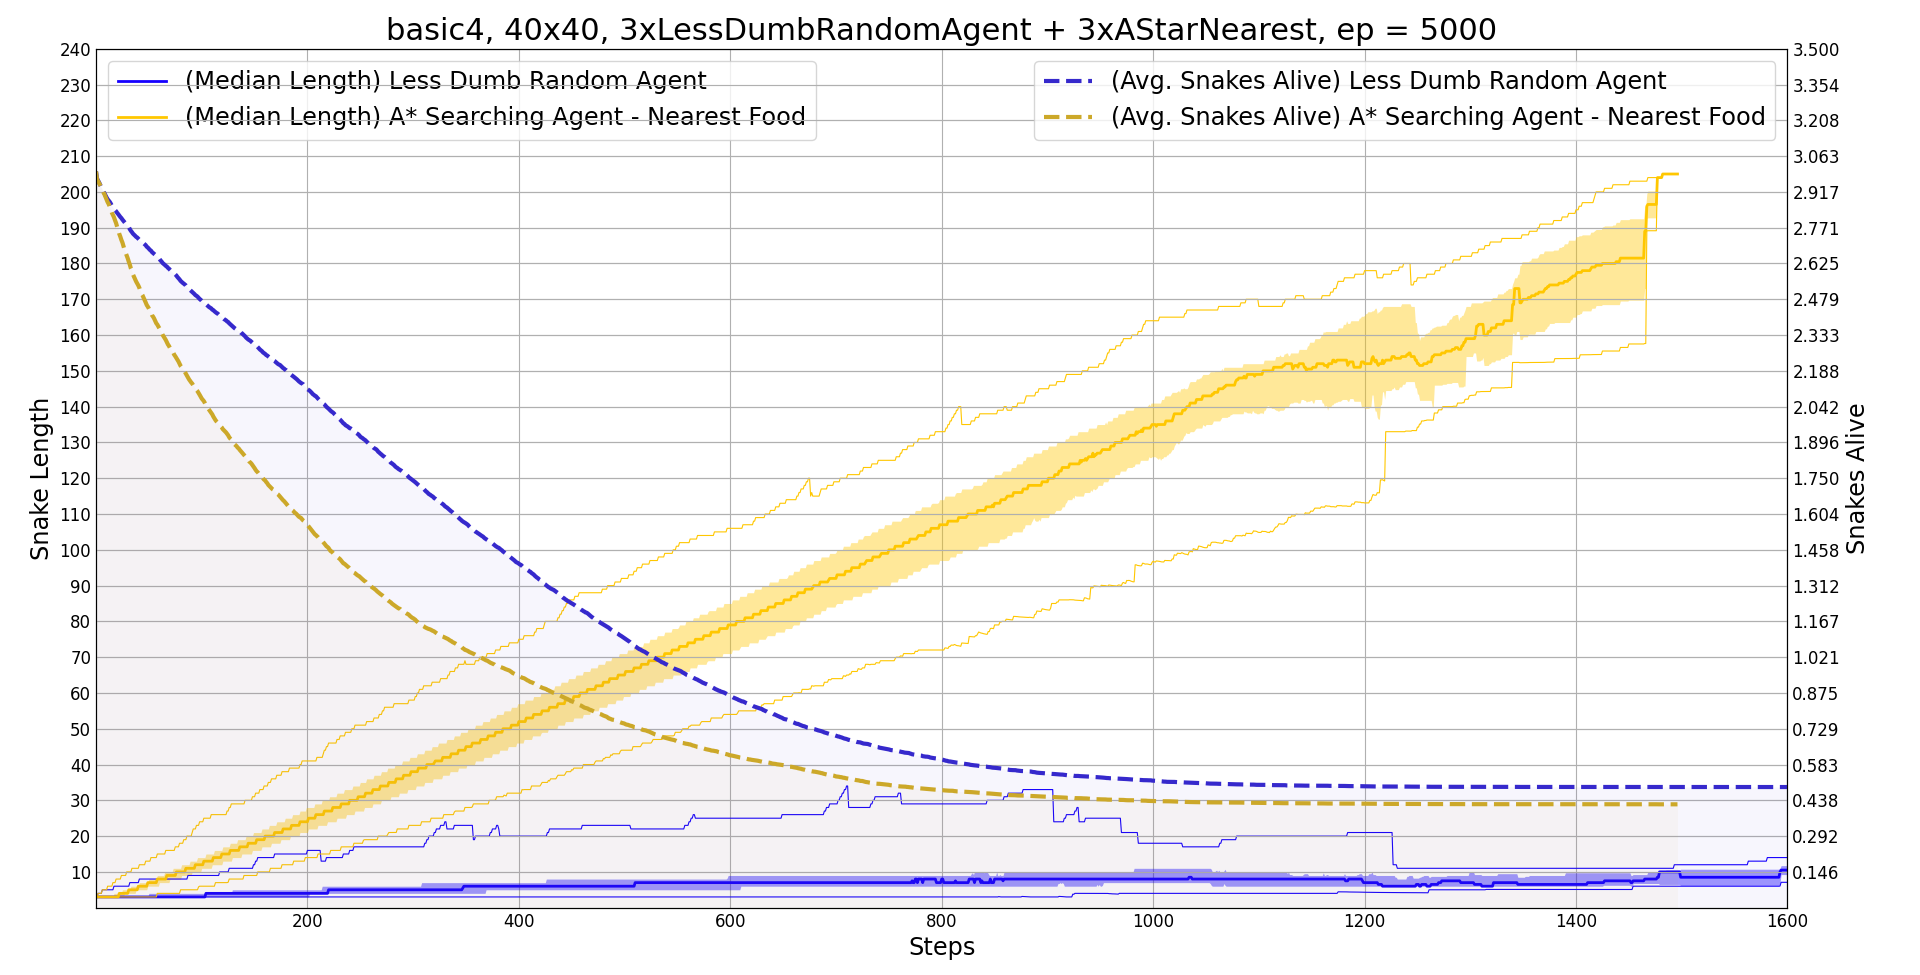
\includegraphics[height=1.6in]{plot_basic4}
\caption{Evolution of the length and population of the Random Agent vs The A* Searcher over time.}
\label{fig_plot_basic4}
\end{figure}

\subsection{Cautious}

The objective with the cautious behavior is to try to predict near agents' next movements,
so that it can avoid moving to the same place (and being removed from the game).
Aside from this behaviour, cautious agents behave in the same way as the Nearest Food searcher\dots
We can see in the images below when a case like, Step: N, occures it will behave in a way so that in "N+2" we should observe the image Step: N + 2.

\begin{figure}
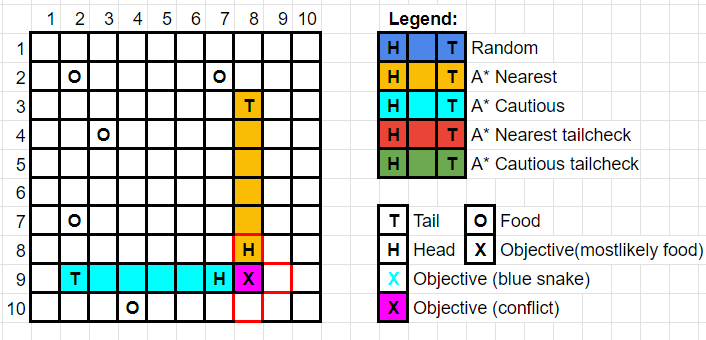
\includegraphics[height=1.6in]{A1}
\caption{Cautious Success Step: N}
\end{figure}

\begin{figure}
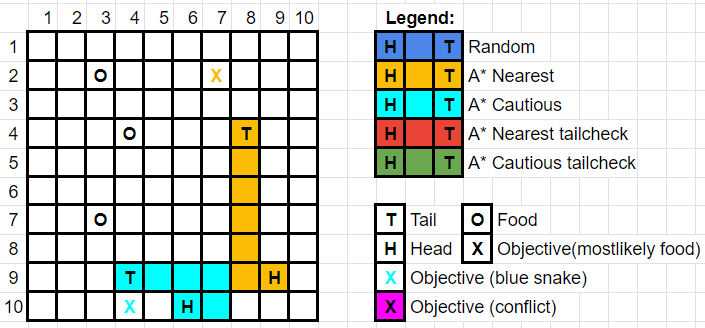
\includegraphics[height=1.6in]{A2}
\caption{Cautious Success  Step: N+2}
\end{figure}

In another hand this behaviour as it's problems since it is based on a prediction if the prediction is wrong that the action won't be favourable\dots
As me can see in the images below, where the cautions behaviour predicts that the yellow agent(A* Nearest) will move to its right, but the yellow agent keeps going forward causing them to be both removed from the episode (head with head colition, figure: Cautious Fail Step: N+1)

\begin{figure}
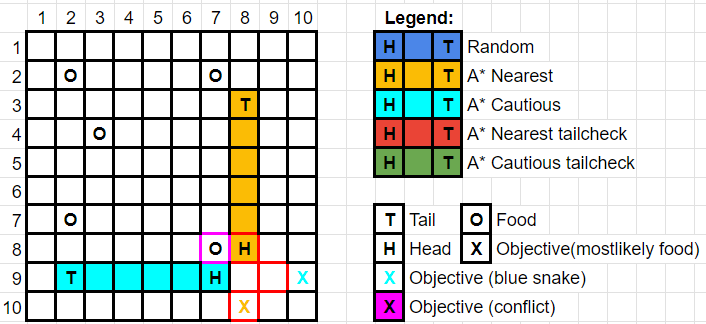
\includegraphics[height=1.6in]{B1}
\caption{Cautious Fail Step: N}
\end{figure}

\begin{figure}
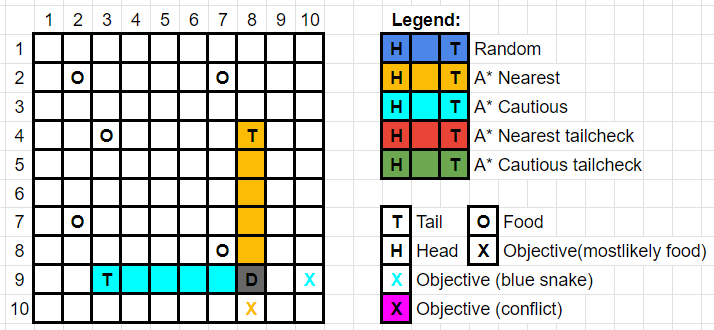
\includegraphics[height=1.6in]{B2}
\caption{Cautious Fail Step: N+1}
\end{figure}

In the following plot we can verify that Cautious behaviour tends to survive more overtime than the nearest food strategie and the size diference between both strategies is not meaningfull.

\begin{figure}
  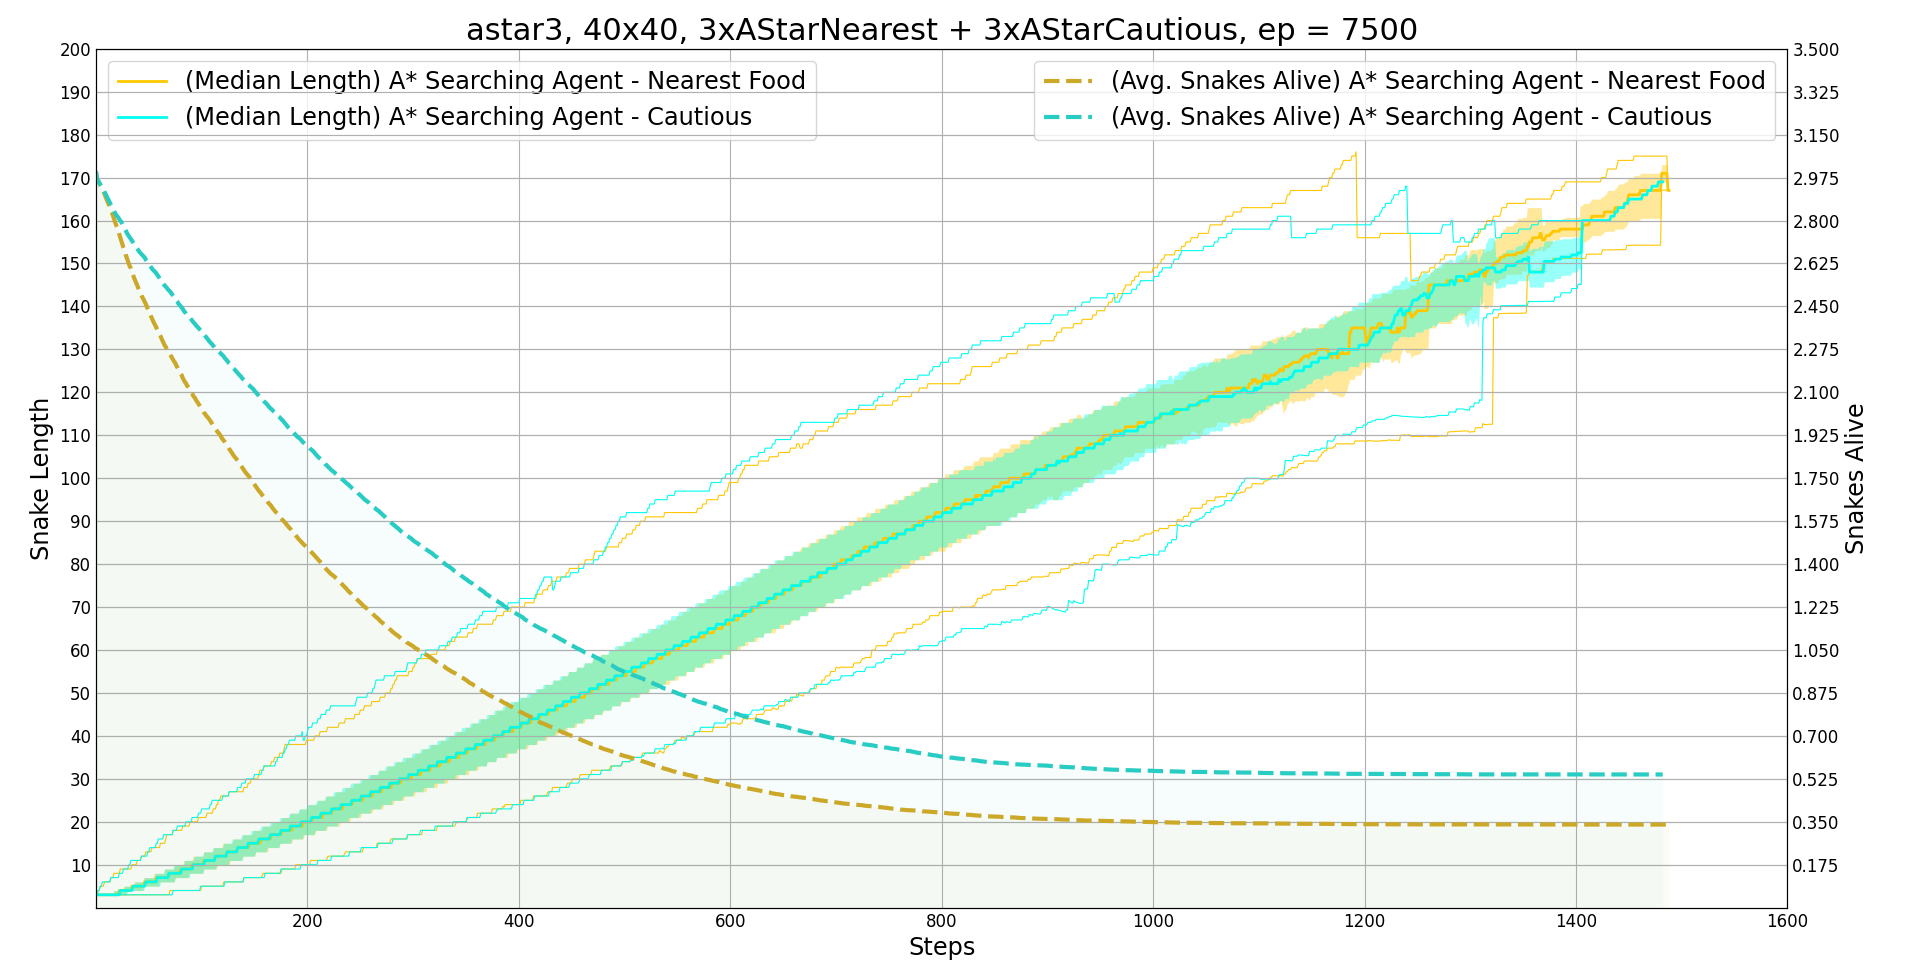
\includegraphics[height=1.6in]{plot_astar3}
\caption{Cautious Fail Step: N+1}
\end{figure}




We decided to go with this behaviour for the cautious agents, but here is an example of the first cautious behaviour we thought, keep in mind this one is not implemented, this hipotetical agent wouldn't use any predictions. It would move base on the place that as 0 risk for him, if faced with potencial risk.
As we see below the cautious agent had an objetive (Cautious Hypothetical Step: N-1) that he gave up (Cautious Hypothetical Step: N) so it could not face in risk, (in this example that made it so that this agent, was kept in the episode)

\begin{figure}
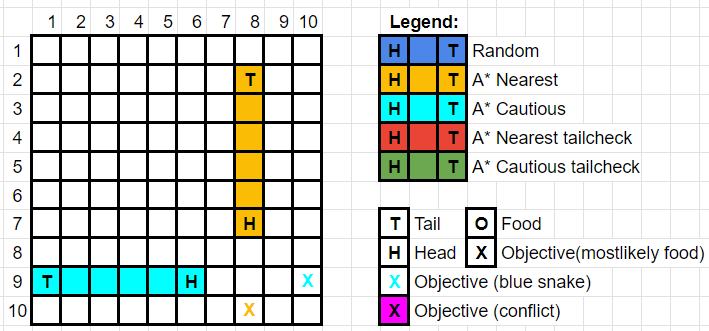
\includegraphics[height=1.6in]{C1}
\caption{Cautious Hypothetical Step: N-1}
\end{figure}
  
\begin{figure}
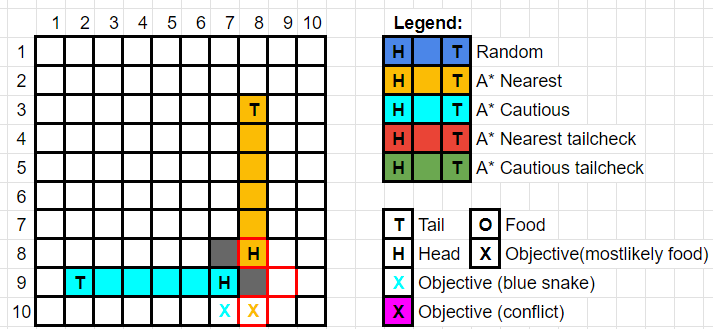
\includegraphics[height=1.6in]{C2}
\caption{Cautious Hypothetical Step: N}
\end{figure}

\subsection{Tail-Checking Search (Don't back yourself into a corner!)}

The objective with the Tail-Checking behavior is to avoid situations where the agent corner themselfs, it does so as the name says by checking if there is still a way to get to is tail even if he does the next movement\dots
We can observe this situation in the first figure below(Tail-Checking Step: N), where this agent will aswer like we can see on the figure (Tail-Checking Step: N+1), so he doesn't trap himself in a corner  


\begin{figure}
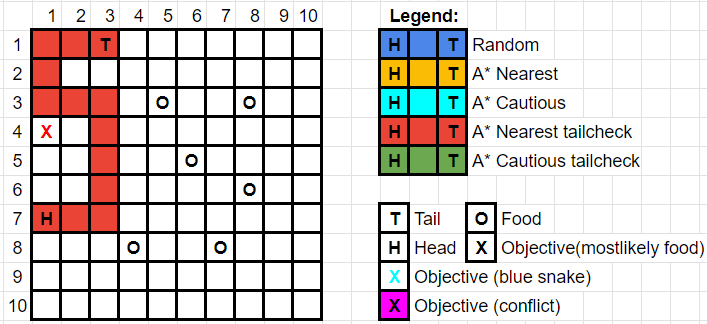
\includegraphics[height=1.6in]{D1}
\caption{Tail-Checking Step: N}
\end{figure}

\begin{figure}
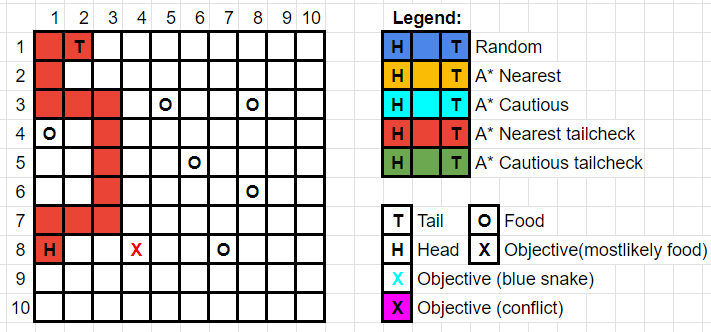
\includegraphics[height=1.6in]{D2}
\caption{Tail-Checking Step: N+1}
\end{figure}

However this search has a flaw since when this is applied in a competitive scenario, it will not work as we see below in the scenario retrated by figures (Tail-Checking Fail Step: N, Tail-Checking Fail Step: N+1) respectivaly\dots
As so with our current implementation in this edge case, we make the agent fallback to a random agent.
  

\begin{figure}
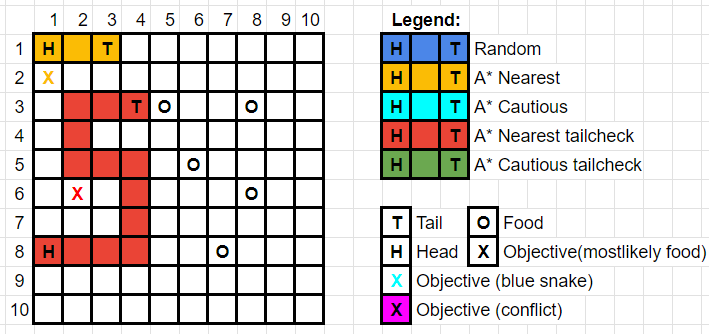
\includegraphics[height=1.6in]{E1}
\caption{Tail-Checking Fail Step: N}
\end{figure}

\begin{figure}
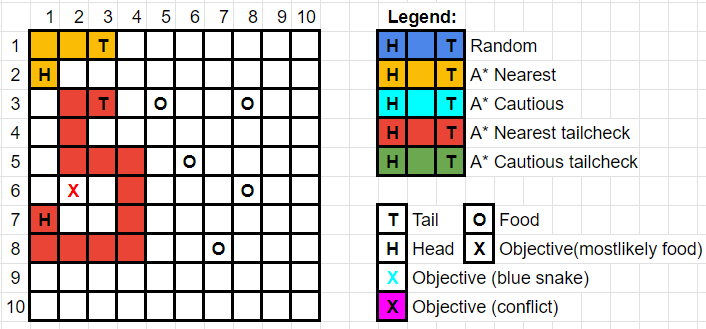
\includegraphics[height=1.6in]{E2}
\caption{Tail-Checking Fail Step: N+1}
\end{figure}

\begin{figure}
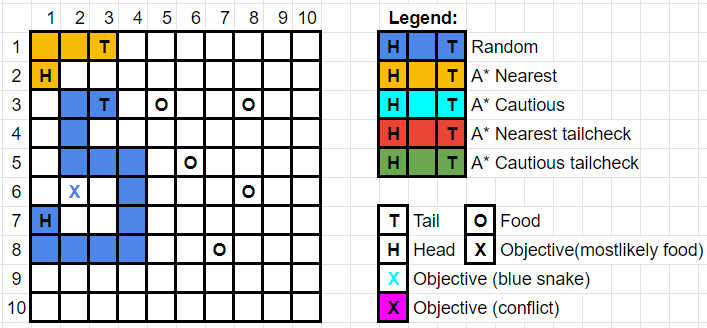
\includegraphics[height=1.6in]{E3}
\caption{Tail-Checking FallBack: N+2}
\end{figure}


The figure below represents the concept of an agent that, when faced with the above scenario, would try to make the longest path posible until it finds a way to its tail, if ever possible\dots

\begin{figure}
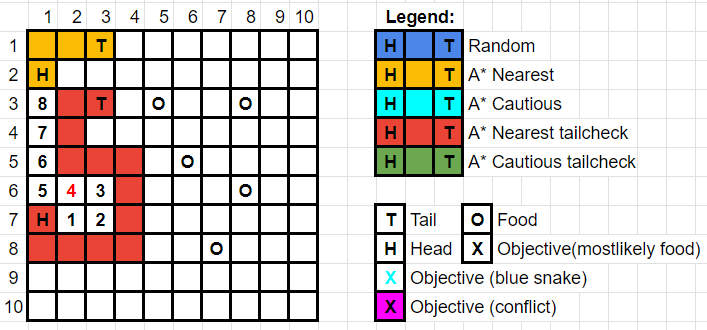
\includegraphics[height=1.6in]{F1}
\caption{Tail-Checking Step: try to make the longest path posible until it finds a way to its tail, if ever possible\dots}
\end{figure}


The plot bellow illustrates a comparision between cautious behaviour and cautious behaviour with tail check:
\begin{figure}
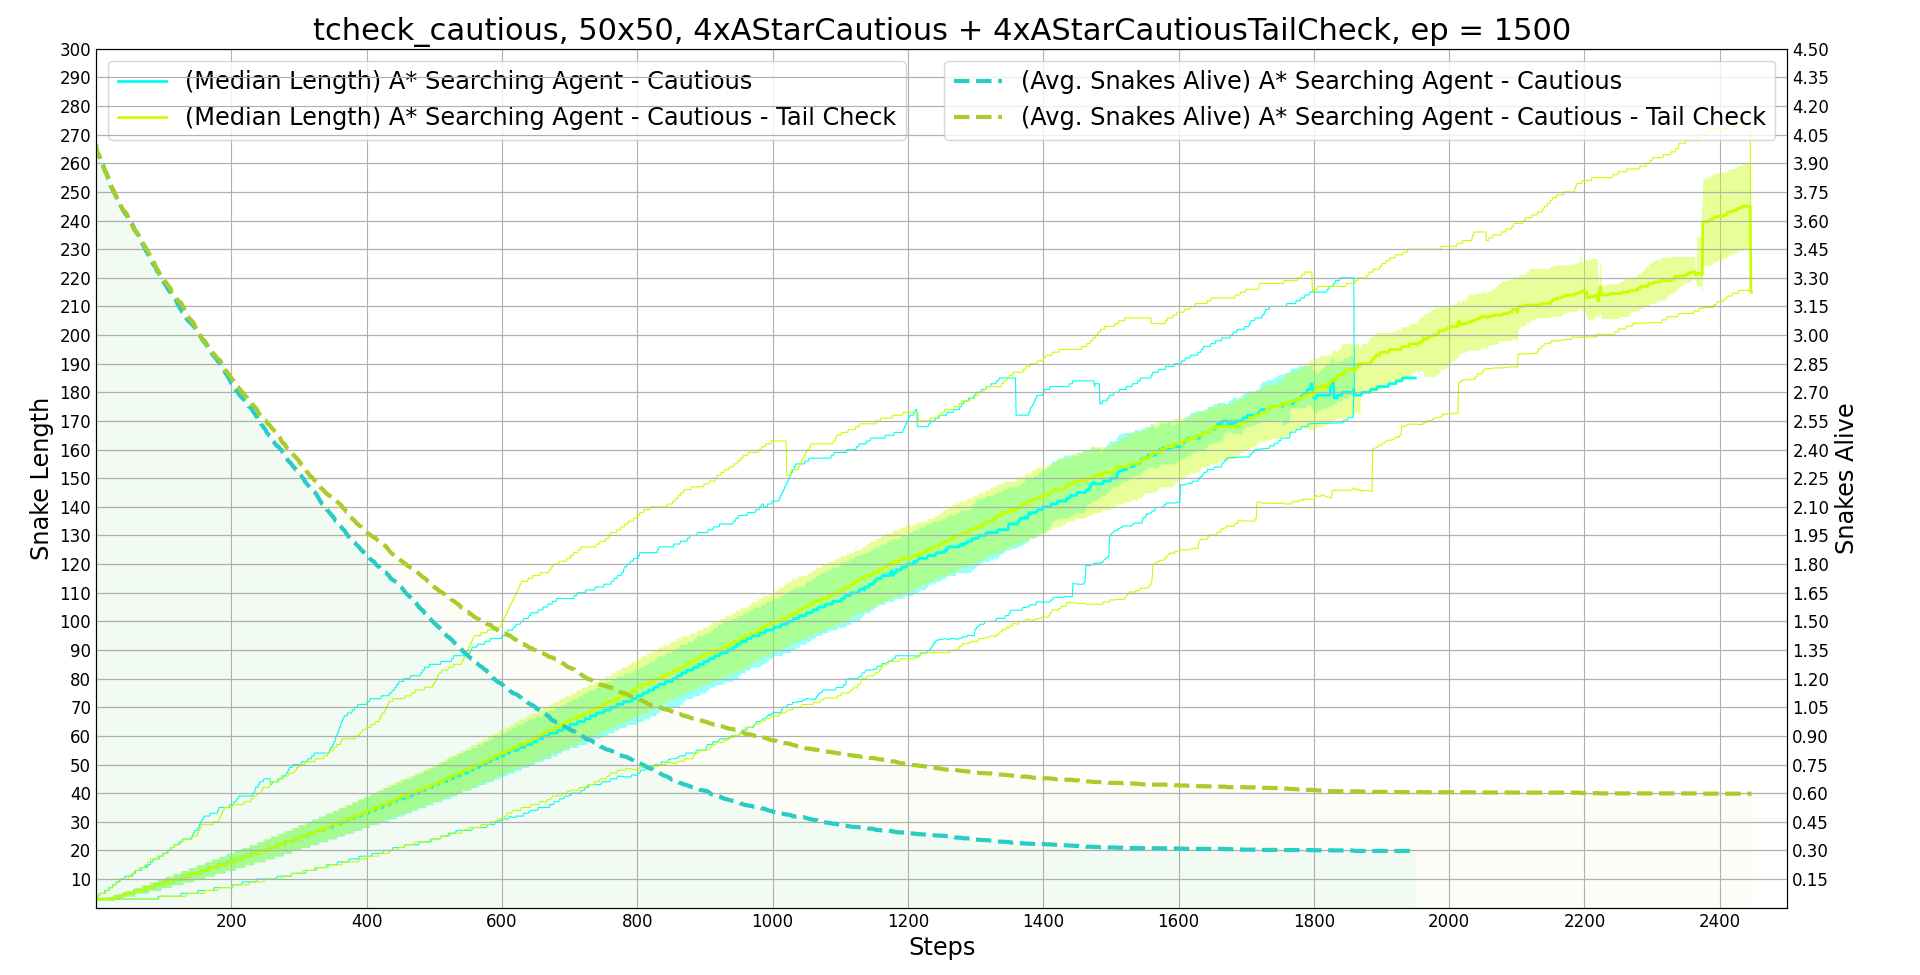
\includegraphics[height=1.6in]{plot_tcheck_cautious}
\caption{Plot cautions and cautions with tail check\dots}
\end{figure}

In this plot (Plot cautions and cautions with tail check), we can clearely observe that, cautious agents with tail check behaviour are surviving 2 times more than the ones without it, and the diference in size between both types of agents is not meaningfull\dots



\section{Conclusion}

With this project, we have reviewed some of the possible strategies that are able to power autonomous agents through uncertainity, either caused by the environment,
other agents, or maybe even themselves. It's been learnt that, long-term, there are certain limitations to running an agent just by feeding it the
information of the moment. It's proven that over time, the agents most well equipped to consider and face uncertainity in the future tend to succeed more.

Those tools do not necessarily need to be a `crystal ball' to predict how the environment will evolve, but educated guesses about their surroundings and what
`makes the most sense' for other agents to do usually help more often than not.



%%%%%%%%%%%%%%%%%%%%%%%%%%%%%%%%%%%%%%%%%%%%%%%%%%%%%%%%%%%%%%%%%%%%%%%%%%%%%%%%%%%%%%%%%%%%%%%%%%%%%%%%%
%% bibliography: see CFP for number of permitted pages

\bibliographystyle{ACM-Reference-Format}  % do not change this line!
\bibliography{references}  % put name of your .bib file here

\newpage

\appendix
%Appendix A
\section{Data and Graphs}

\begin{figure}
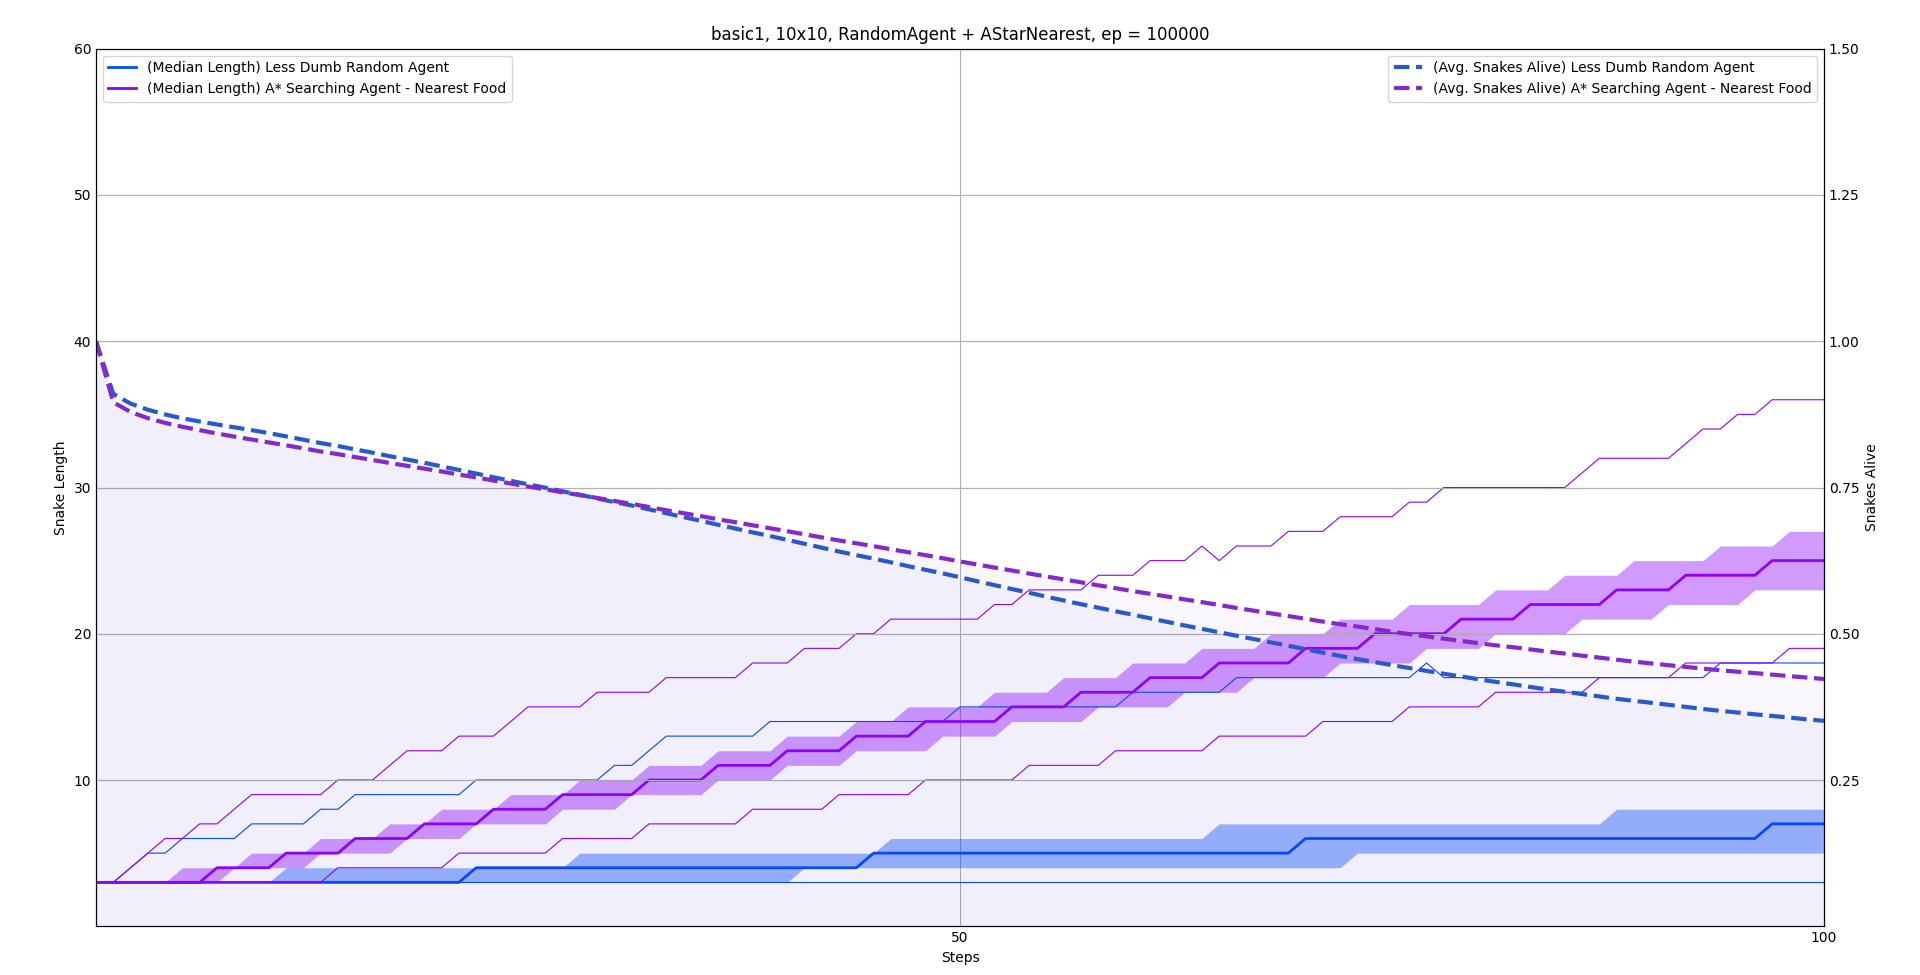
\includegraphics[height=1.6in]{plot_basic1}
\end{figure}

\begin{figure}
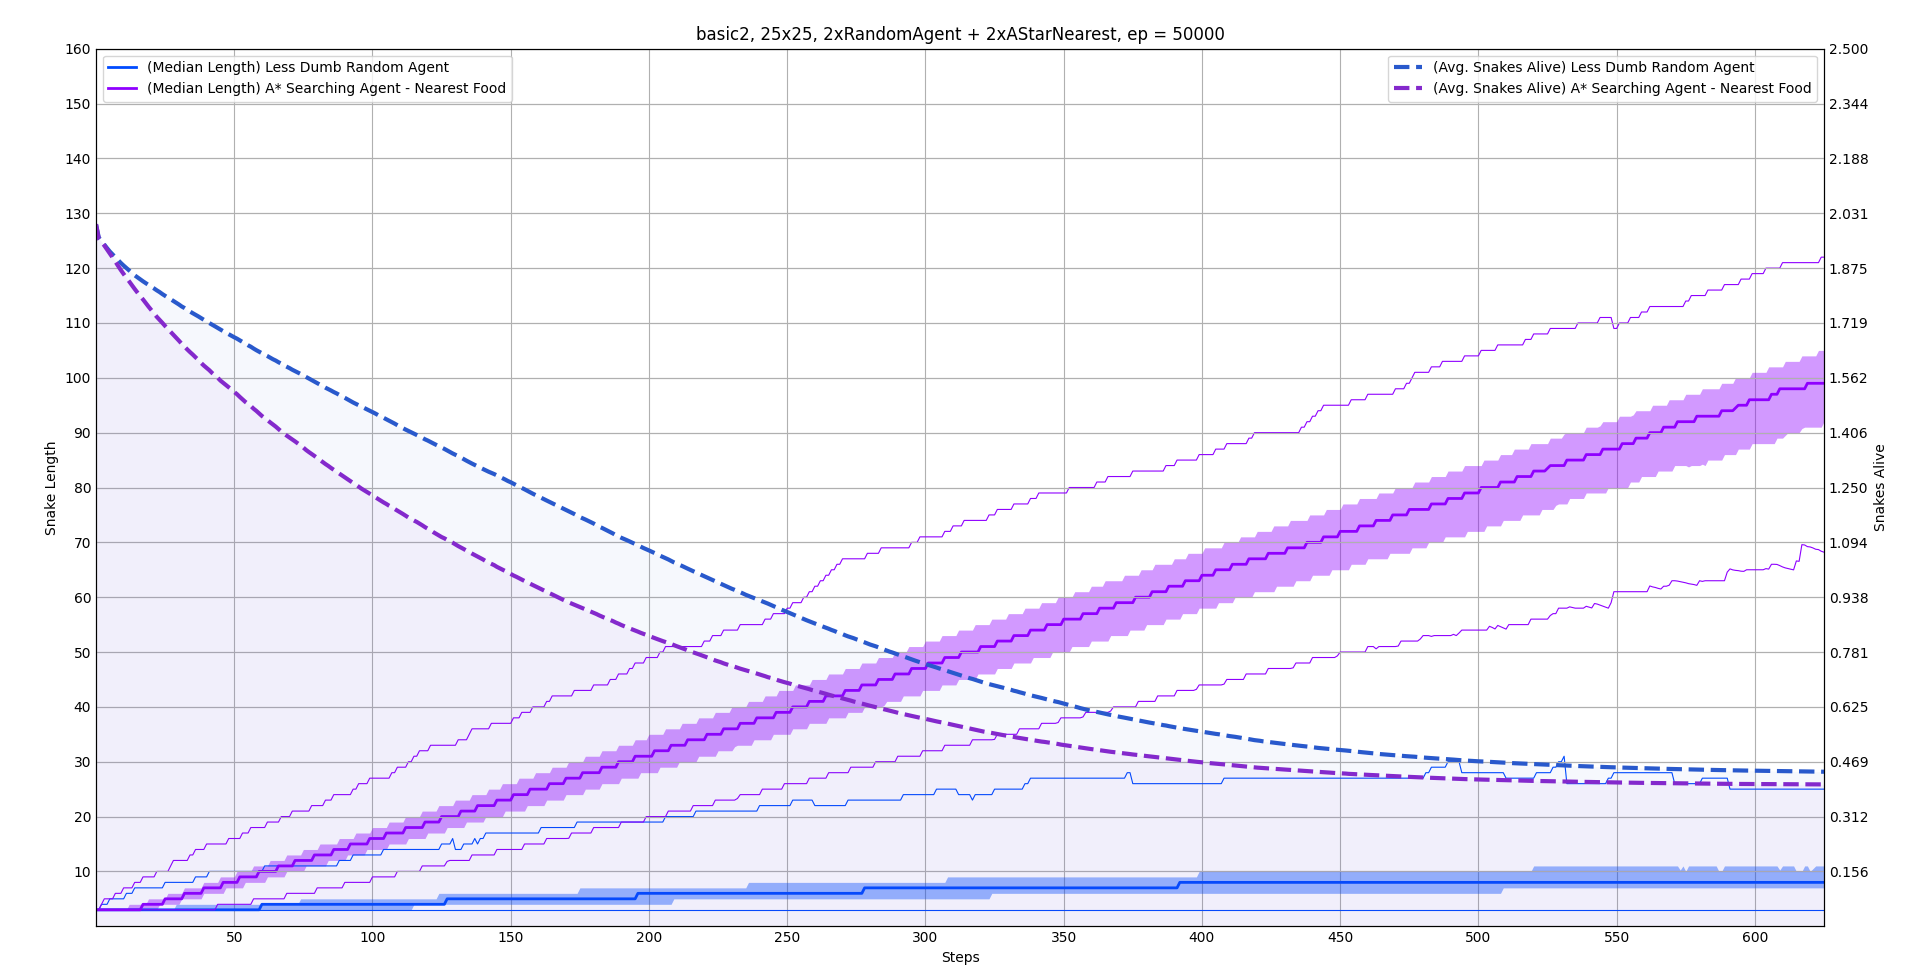
\includegraphics[height=1.6in]{plot_basic2}
\end{figure}

\begin{figure}
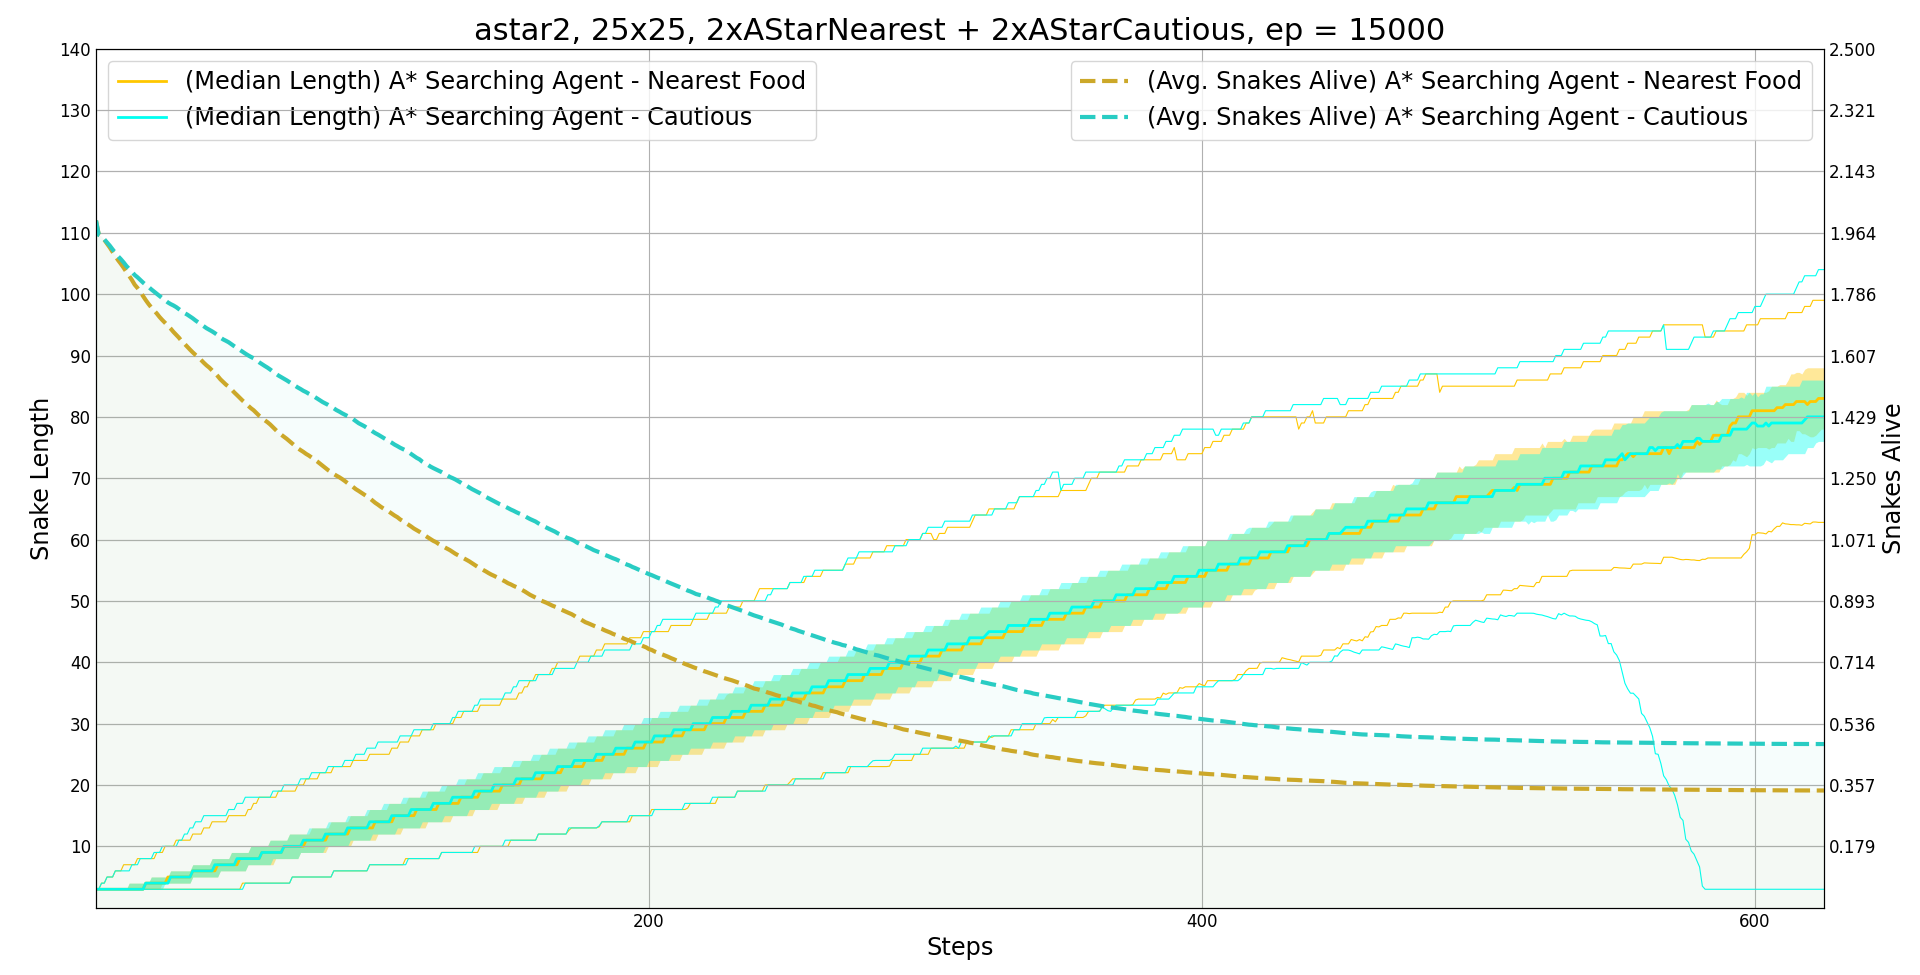
\includegraphics[height=1.6in]{plot_astar2}
\end{figure}

\begin{figure}
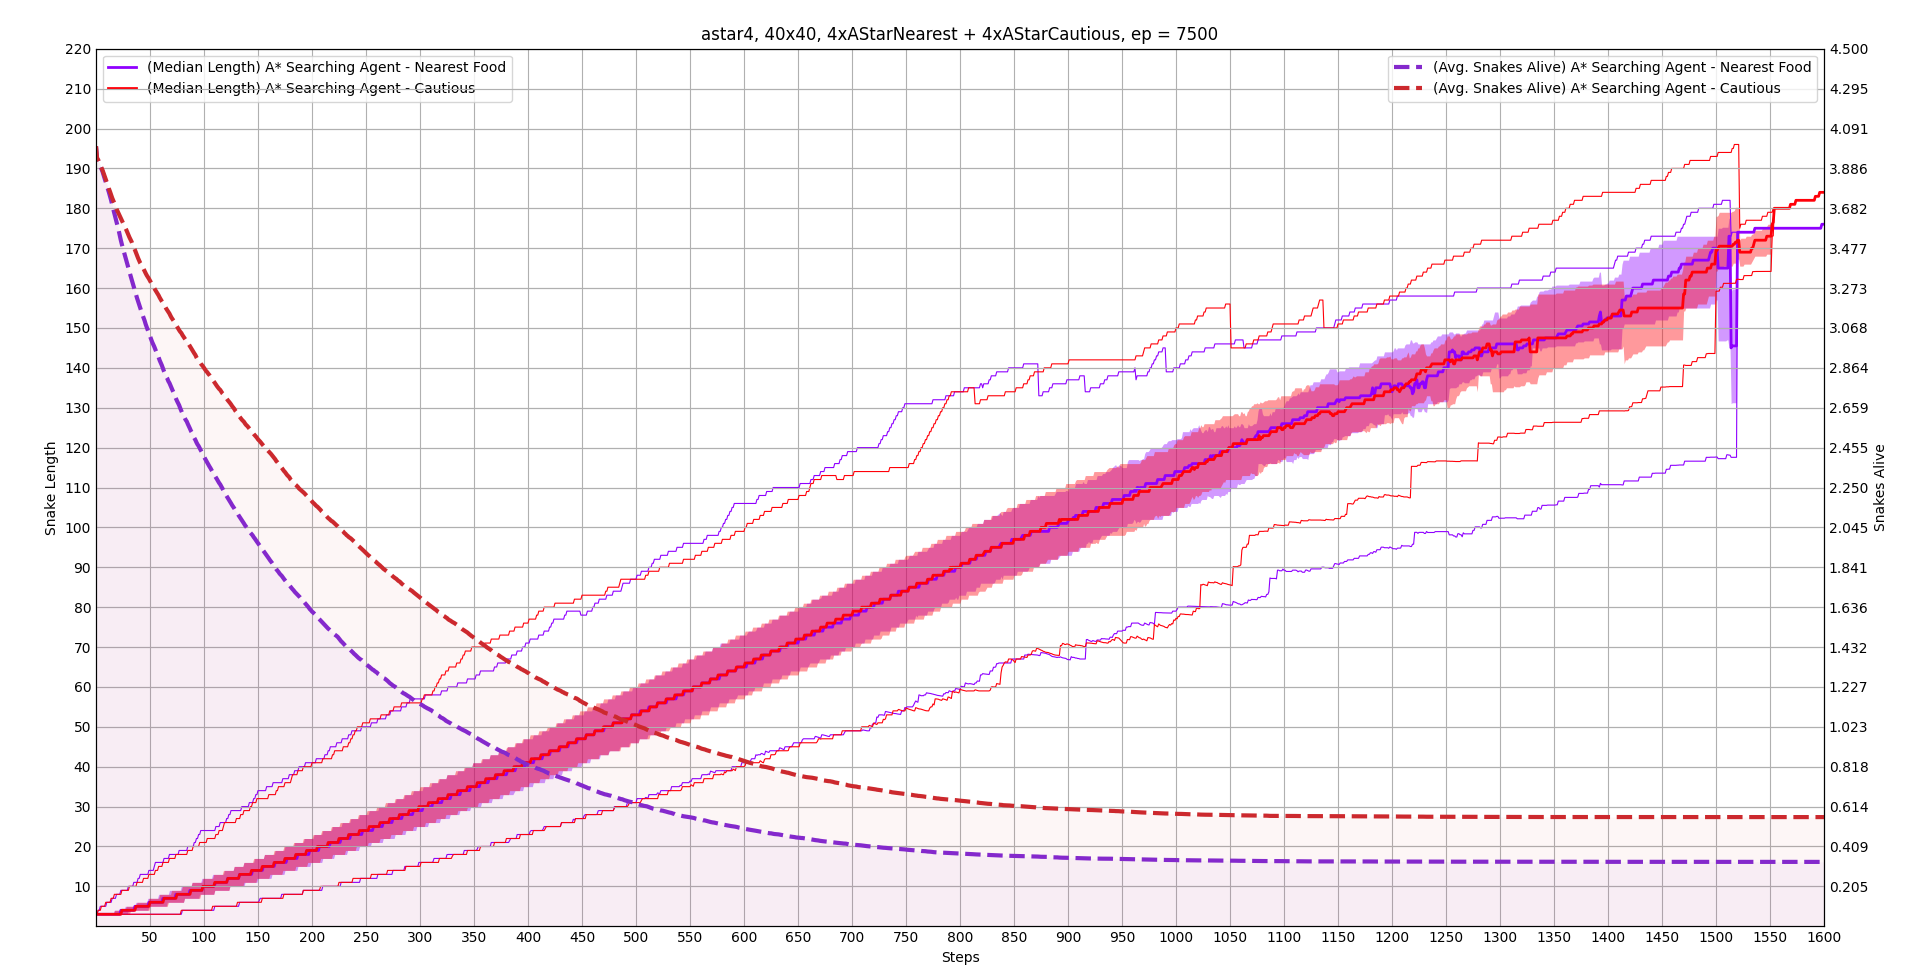
\includegraphics[height=1.6in]{plot_astar4}
\end{figure}

\begin{figure}
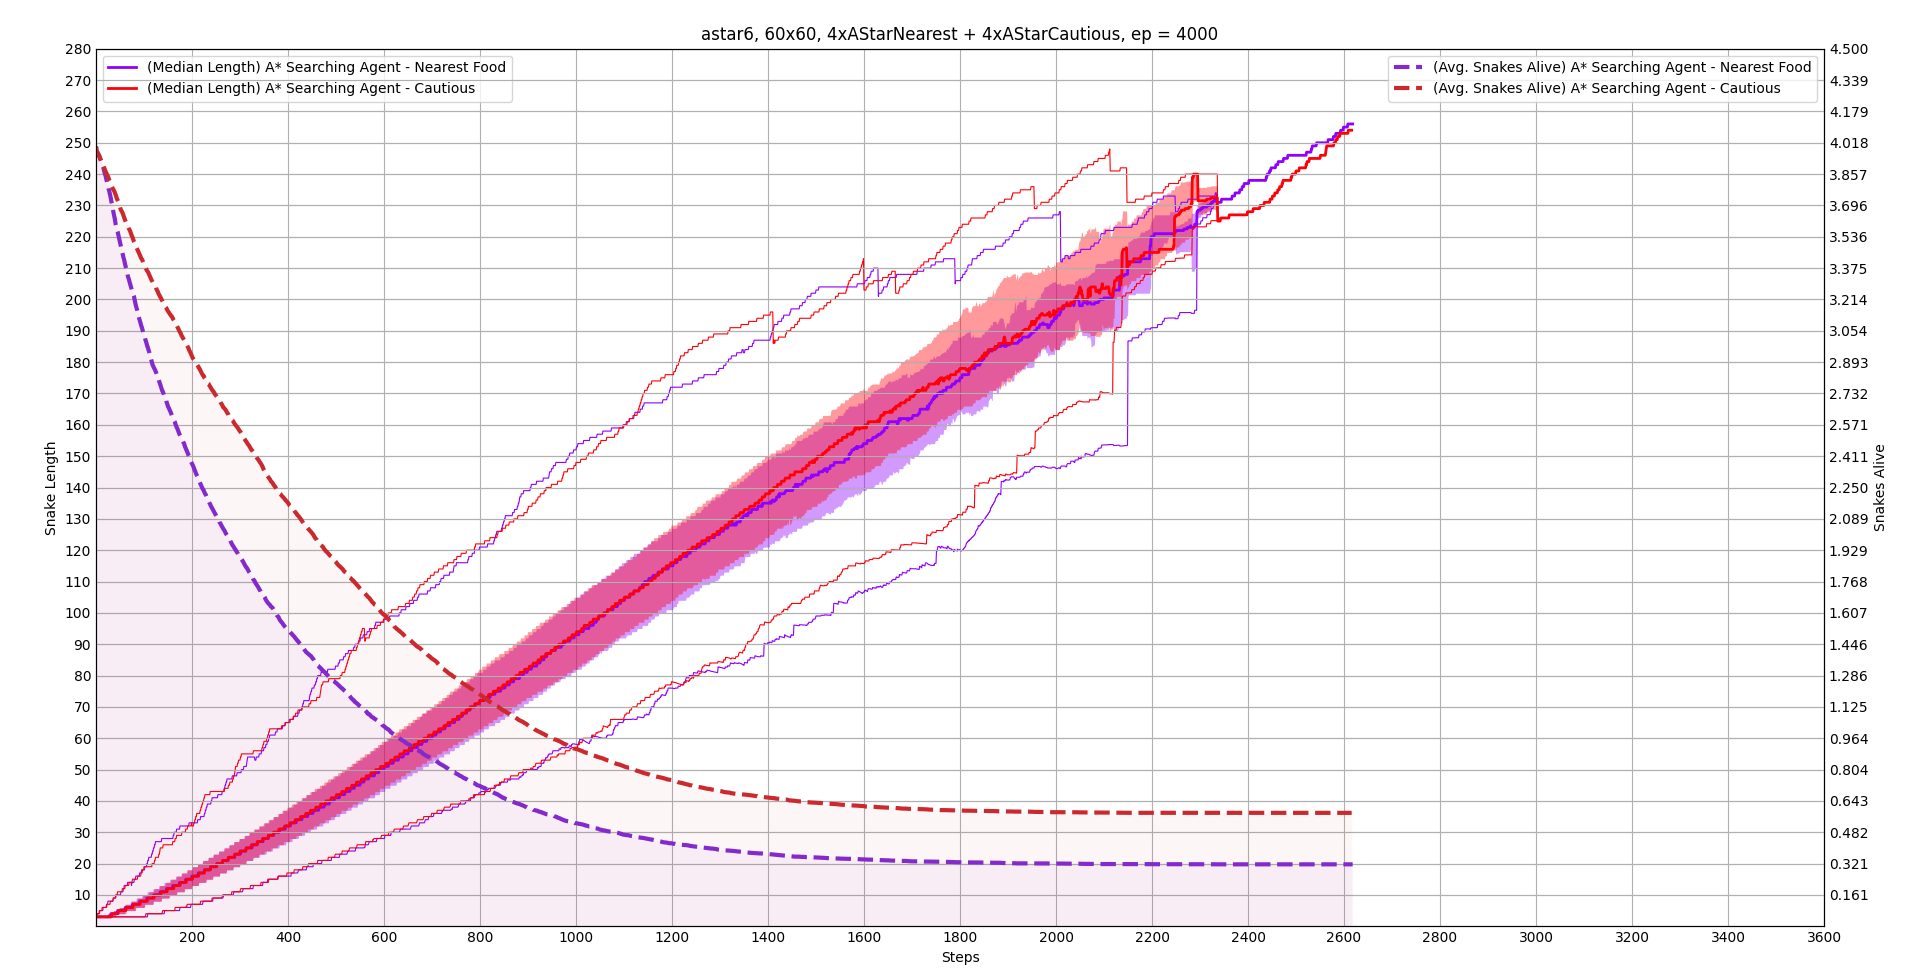
\includegraphics[height=1.6in]{plot_astar6}
\end{figure}

\begin{figure}
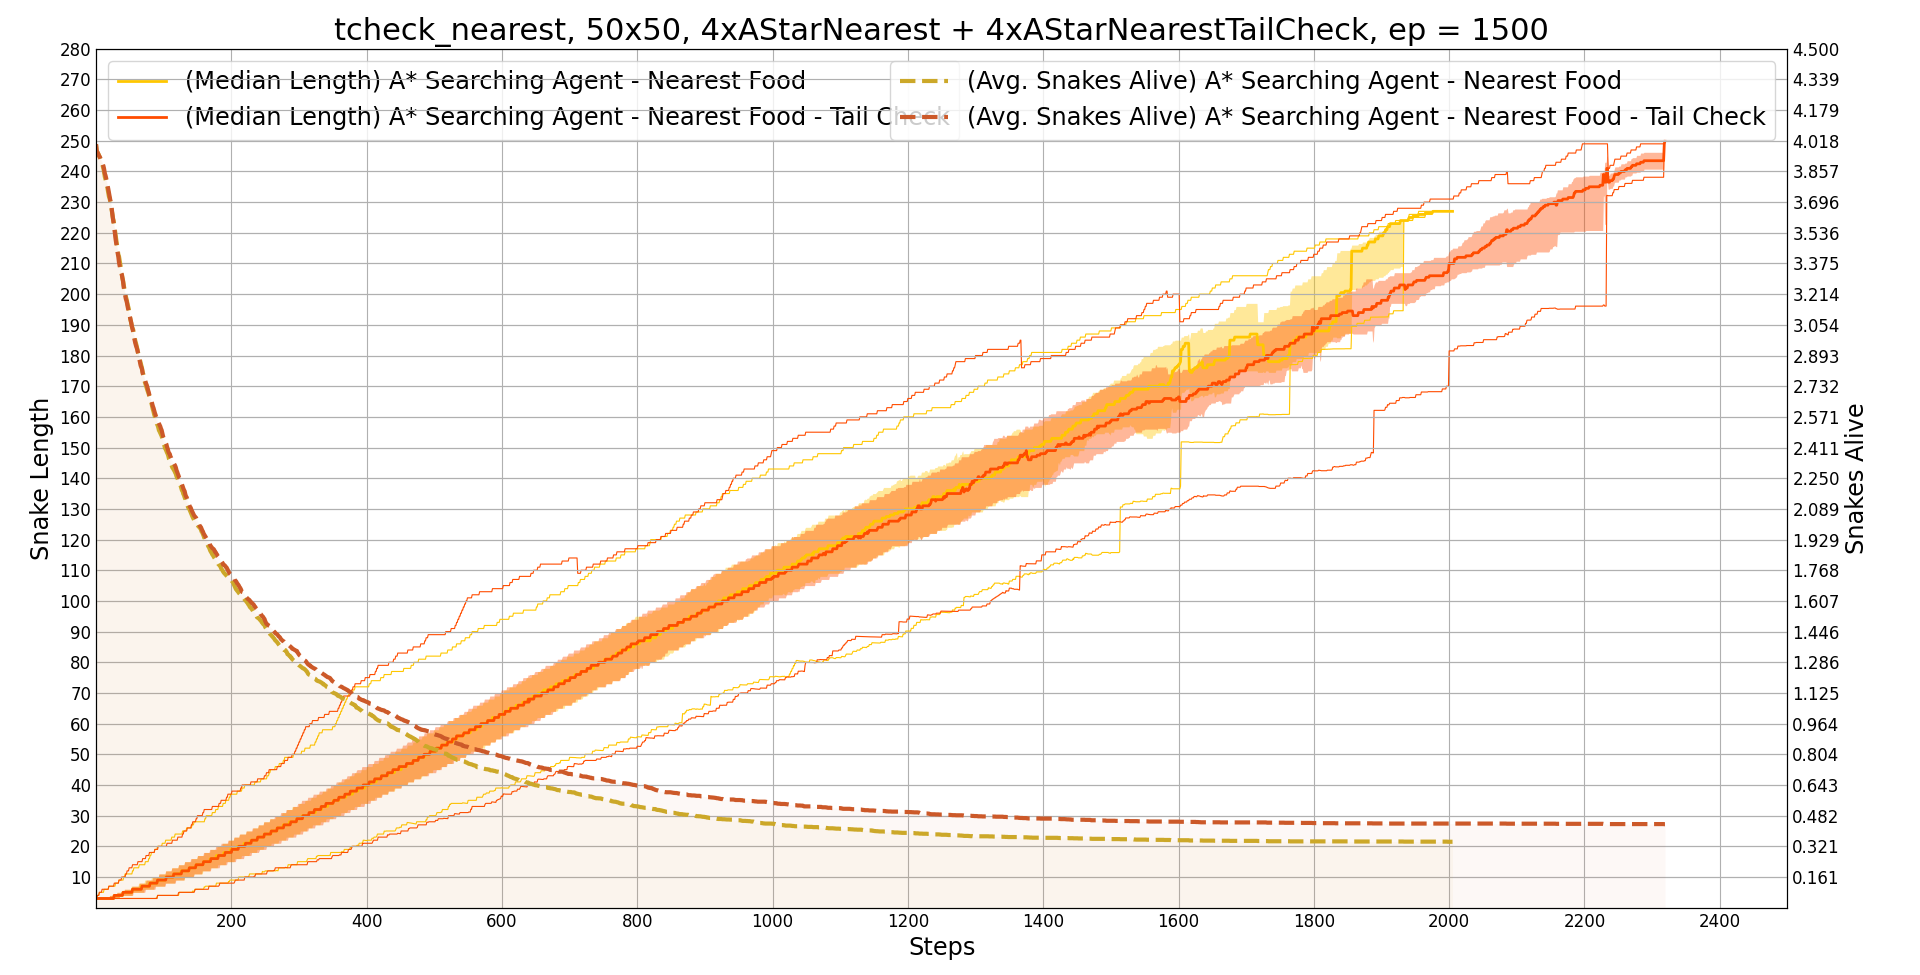
\includegraphics[height=1.6in]{plot_tcheck_nearest}
\end{figure}

\begin{figure}
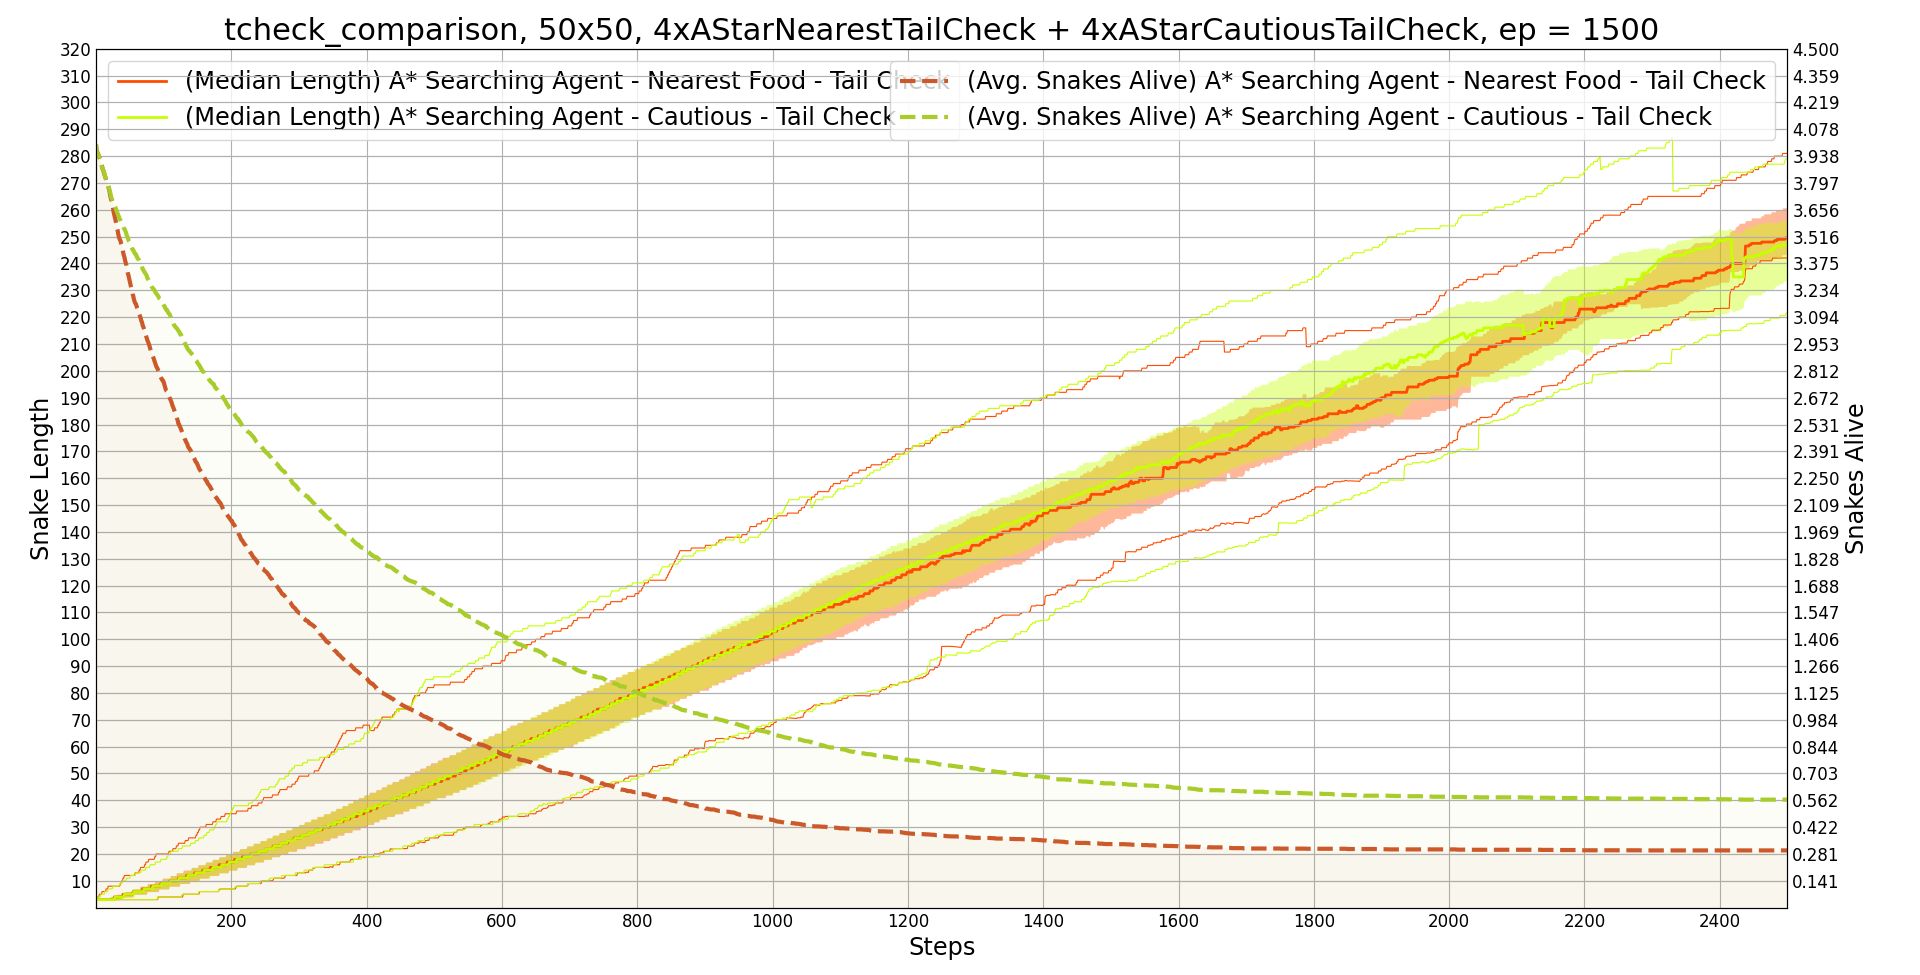
\includegraphics[height=1.6in]{plot_tcheck_comparison}
\end{figure}


\end{document}
